% !TEX root = ../main.tex

\chapter{课题背景和研究意义}

本章节将介绍CIS芯片的前端设计和深度学习网络软硬件发展的背景,讨论两者之间的联系以及
研究的内容和意义。

\section{国内外研究现状}

\subsection{ASIC与CIS芯片}
%TODO 描述ASIC的基本概念
%TODO 描述CIS芯片的基本概念
CMOS Image Sensor(CIS)就是一种基于CMOS工艺制造的图像传感器。
我们现今常见的照相机、安防摄像头、手机摄像头内使用的图像传感器大多都是采用的CIS芯片。
CIS芯片也属于一种专用集成电路(ASIC)。
专用集成电路(ASIC)的全称是Application Specific Integrated Circuit,它是一种用于特定场景或者用途的芯片。
ASIC设计对任何公司来说都是一项高难度的挑战。  

近年,CIS芯片市场供不应求,技术飞速发展。CMOS图像传感器是一种典型的固体成像传感器,与CCD有着共同的历史渊源。
CMOS图像传感器通常由像敏单元阵列、行驱动器、列驱动器、时序控制逻辑、AD转换器、数据总线输出接口、控制接口等几部分组成, 这几部分通常都被集成在同一块硅片上。
其工作过程一般可分为复位、光电转换、积分、读出几部分。  
索尼在2012年推出了全球首款用于消费电子产品的堆叠芯片CIS相机系统(CIS+ISP)。
在2017年的ISSCC大会上,索尼又发布了他们的一款三层堆栈式CIS。[1] %引用
其结构为:顶层的图像感知层、中间的DRAM层和底层的逻辑电路层(CIS+DRAM+ISP)。
堆栈式CIS芯片成为了发展趋势。
随着各厂商的设计能力与工艺的提升,越来越多的IP被集成到CIS芯片的堆栈中,使得现今的CIS芯片功能更加强大和复杂。
由于堆栈式设计的存在,使得我们将深度学习神经网络的运算模块叠加在CIS芯片中成为可能。  

\subsection{深度学习、残差网络和脉动阵列}
想要实现深度学习神经网络算法的硬件加速,就先要对深度学习神经网络算法有所了解。
% 简述DL的发展,例举出最经典的一些算法。
卷积神经网络(Convolutional Neural Networks, CNNs)和深度神经网络(Deep Neural Networks, DNNs)是目前最先进的两种机器学习算法之一。%引用
它们都属于多层感知器(MLPs)家族,可能包括四种类型的层:卷积层、池化层、归一化层和分类器层。%引用
回顾深度学习算法的发展史,始于LeNet识别了10个手写的数字。
它是一种广泛用于文档识别的卷积神经网络,由两个卷积层、两个池层和三个分类器层组成。
卷积层实际上是一种滤波器。它可以用来识别输入的特征图的某些特征。
每个局部滤波器都有一个$K_x$x$K_y$尺寸的核,用来处理卷积窗口。
这个卷积窗口将捕获一个输入特征映射中的$K_x$x$K_y$尺寸的输入神经元。
局部滤波器的2D阵列产生一个输出特征映射。
其中的每一个局部滤波器对应一个输出神经元。

% 简述ResNet
% TODO 简述ResNet18的网络结构
ResNet18由4个主要的残差层组成。
整个网络的开头,由7x7的卷积核做卷积运算和3x3的最大池化。
卷积运算有64个输出的通道。设定的步长是2,填充的边框是3。
最大值池化的步长是2,填充的边框是1。
最后输出的图像尺寸是112x112

之后是四个包含两个BasicBlock来做运算的残差层。
每个BasicBlock中都有两个3x3的卷积运算。
它们的深度不同,分别是64、128、256和512。
ResNet可能使用两种不同的残差单元。一种是BasicBlock,用于ResNet18和ResNet34这种浅层网络。
另一种是Bottleneck,用于50层及以上的ResNet。

% 实现哪一种深度学习算法
本课题中,将要通过设计专用的硬件加速器来进行ResNet18的前向计算。
因此,这一小节将分析ResNet18所涉及到的所有基本运算。


\subsection{用于深度学习运算的硬件}
2012年多伦多大学基于AlexNet开发的SuperVision在ImageNet处理上实现了极大的提升是近年的一个里程碑。%引用
感知时代也始于2012年。之后谷歌在几千台普通机器上进行了出色的并行CPU有损更新研究。
在这之后的2014年,VGGNet与GoogLenet相继诞生,专为神经网络设计的硬件在90年代初诞生。
CNAPS(1990),它带有64个处理单元和256kB内存,可以在8/16位条件下达到1.6 GCPS的速度(CPS是指每秒连接次数 / connections per second)或在1位条件下达到12.8GCPS的速度。%\cite{ref1}   

随着大数据和深度学习的发展,用于相关领域的硬件发展趋势也受到业内人士以及专家们的广泛关注。
在半导体领域,2019 ISSCC大会于2月17—21日在美国旧金山开幕。
Facebook首席AI科学家Yann LeCun在会上发表了主题演讲”深度学习硬件:过去、现在和未来“,详细介绍了深度学习研究的发展将如何影响未来硬件架构。%引用  

深度神经网络在图像的识别、分类、检测和分割等领域起到了非常重要的作用。
在各种DNN的网络结构中,卷积神经网络是最常见的一种。
常见的硬件加速方案中,主要有CPU、GPU、FPGA和ASIC。
如图\ref{fig:silicon_alternatives}所示,这些半导体器件在应用灵活度和能效比两方面的关系成反比。  
\begin{figure}[htbp]
    \centering
    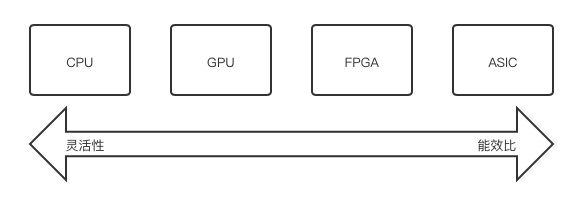
\includegraphics[width=15cm,height=4.5cm]{figures/silicon_alternatives.png}
    \caption{半导体器件能效比与灵活度关系示意图}
    \label{fig:silicon_alternatives}
\end{figure}

CPU和GPU的方案依赖于指令集和编译器的支持。
在实际应用中,GPU无论在训练深度学习神经网络的模型,还是图像识别或分类等深度学习的应用上,都比CPU更具有优势。
GPU相比CPU主要具有以下三点优势:
\begin{enumerate}
    \item 提供了更多可供并行计算的基础计算单元。典型地,这里的并行可以理解为单次执行多条指令的算法。
    \item 防存速度更快,因为GPU的每个核都拥有自己独立的cache;
    \item 一般的,GPU比CPU具有更高的浮点数运算能力。
\end{enumerate}
不过这两者的硬件平台都不是专用于深度神经网络运算的。
FPGA是可编程逻辑门电路,这种方案既可以实现算法的硬件加速,又可以不用支付ASIC后端开发和流片的成本。
ASIC作为一种专用的硬件加速方案,在性能和功耗,特别是能耗比上,是其他几种方案都无法相比的。
一般地,这种芯片被称为嵌入式神经网络处理器(NPU)。

近年,通过FPGA和ASIC实现硬件神经网络加速器的方式在功耗和性能上展现出了巨大的优势。
工程师们还想要进一步降低功耗和提升性能受到存储器访问的限制。
本课题关注的是图像识别的应用。用于该应用的最先进的神经网络算法就是卷积神经网络,它的一个重要特性就是权重在神经元之间共享。
这种特性大幅减少了在神经网络的运算中所使用的内存,允许我们在SRAM中完全映射一个卷积神经网络,并且避免访问DRAM来读取权重值。
而CIS芯片的数据通路具有流水线的特性,使得这种设计具有通用的深度学习加速器不具有的并行运算能力。
另外,加速器本身处在数据通路中,将会进一步减少为了读取输入数据和写入输出数据而进行的DRAM访问。   

与机器学习或深度学习相关的边缘计算领域也在今年得到了长足的发展。
例如:由Pete Warden 与 Daniel Situnayake在2019年提出的TinyML就是在毫瓦功率的微处理器上,实现机器学习算法、工具和技术。%引用
这一技术是基于Tensorflow Lite在微控器上的软件框架和硬件环境而来的。
一般来说,它只需要几十千字节的存储空间。  

在CIS的领域,物联网中的感知节点数量持续快速增长,产生海量数据。
到2032年,从感官节点产生的信息相当于1020bit/s,远大于人类感官总吞吐量。%引用
尽管5G网络或是将来的6G网络会为物联网提供高速传输和大带宽。
因此,近传感器和传感器内计算范式的概念被提了出来。
通过它们在传感器和运算单元之间的位置来定义它们输入哪一种类型。
因为感知功能是在有噪声的模拟域中实现的,使用集成在同一域中的模拟处理器来处理传感器数据是非常理想的,这种类型就是传感器内计算。
这种高效率运算系统避免了数模转换,减少了延迟和功耗。




\subsection{ShiDianNao与谷歌TPU}
近几年,市场上的NPU百花齐放。
几乎所有市场上的旗舰手机SoC都嵌入了NPU。
由于各家厂商嵌入在SoC中的NPU各不相同,因此性能和功耗也是天差地别。
各个厂家也是对这个新ip讳莫如深。
公开可查到的有谷歌TPU和寒武纪的Diannao系列。
它们的设计思想可以作为后续设计的参考。
当前情况下,寒武纪的Diannao系列显得比谷歌的TPU更开放一些。
寒武纪开放了其指令集Cambricon和相应的工具链或者是云服务。
同时,寒武纪的Diannao系列作品的论文也非常完整,特别是ShiDianNao对本课题有非常大的借鉴意义。
谷歌TPU方面,我们只能通过Google Colab服务来使用云端的TPUs。
在最新款的谷歌手机上,名为Google Tensor的SoC芯片内置了Google edge TPU来加强机器学习的运算能力。
但谷歌没有开放相关的SDK,因此可以相信这个TPU只是给设备原生的一些应用使用的。


\subsubsection{ShiDianNao和Cambricon}
%TODO 简单介绍shidiannao和Cambricon的原理
在国内,寒武纪的DianNao系列产品可谓是深度学习处理器的先驱。
DianNao是在2014年寒武纪深度学习处理器的开山之作。
它可以被看作是此系列处理器的硬件设计基础。
后来的的DaDianNao、ShiDianNao、PuDianNao则分别适用于服务器端的高性能计算、设备端边缘计算和更加泛化的机器学习算法。
其中,DianNao、DaDianNao和PuDianNao采用了流水线式乘加树的结构。  %引用   


% ShiDianNao的整体架构描述。
% ShiDianNao的整体架构贴图。
% ShiDianNao的DL加速单元架构描述。
% 上述架构的贴图
ShiDianNao是一个放置在CMOS或CCD传感器旁的CNN加速器。
它有特定的数据访问模式来避免DRAM的读写访问。
这是的ShiDianNao具有以前最先进的神经网络加速器的60倍的能效比。
它在65纳米的布局下,面积为4.86 $mm^2$,功耗仅为320 mW,但仍然比高端GPU快30倍。

\begin{figure}[htbp]
    \centering
    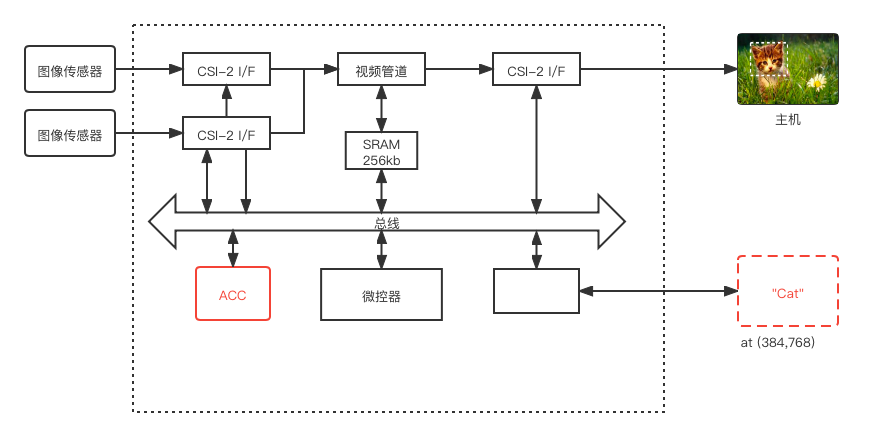
\includegraphics[width=15cm,height=8cm]{figures/ShiDianNao_arch.png}
    \caption{ShiDianNao的架构图}
    \label{fig:shidiannao_arch}
\end{figure}
ShiDianNao的架构设计如图\ref{fig:shidiannao_arch}所示,在整个SoC上类似于一个挂载在总线上的外设。
加速器有两个功能单元,一个NFU用于调节基本神经元操作(乘法、加法和比较),另一个ALU用于执行激活函数计算。
它的核心模块是NFU(神经功能单元)。
NFU是由$P_x$×$P_y$个处理元素(PE)组成的2D网络。
与DianNao系列的其他产品相比,NFU天然地适合2D特征图的拓扑结构。  
神经元(PE)映射的直观方法是将一块$K_x$×$K_y$ PEs($K_x$×$K_y$是内核大小)分配给单个输出神经元,同时计算所有突触。
但是ShiDianNao中,优化了计算方法。
它将每个输出神经元映射到单个PE,并在连接到同一输出神经元的输入神经元(即突触)之间共享每个PE。  
NFU不能覆盖CNN中的所有计算原语,因此ShiDianNao需要一个轻量级ALU来补充PEs。
ALU实现了16位定点算术运算符,包括除法(用于平均池化和归一化层)和非线性激活函数,如tanh()和sigmoid()(用于卷积层和池化层)。

\subsubsection{谷歌TPU的脉动阵列}
%TODO 简单介绍谷歌TPU的脉动阵列原理。
% TPU的架构设计描述
% TPU的架构设计图
如图,主机通过PCIe总线发送TPU指令到指令缓冲区。其内部模块通过256位宽的数据通路连接。
谷歌TPU的核心部件是图中右侧的矩阵乘法单元。
它包括了256x256个乘加器,可以执行8位无符号和有符号整数乘法和加法。
在计算得到16位无符号或有符号整数后,保存在32位累加器中。
TPU在运算时的核心思想是利用脉动阵列来减少缓冲区和SRAM的读写访问。
它的理念是保持矩阵乘加单元一直工作。
TPU拥有4级流水线。同时设计了一组指令来控制访存和运算。其中每条指令在单独的阶段执行,主要的指令如下:
\begin{enumerate}
    \item Read\_Host\_Memory
    \item Read\_Weights
    \item MatrixMultiply/Convolve
    \item Activation
    \item Write\_Host\_Memory
\end{enumerate}
设计遵循了解耦访问和执行的原则。
因此在发出Read\_Weights指令之后,MatrixMultiply就可以开始执行,不需要等待Read\_Weights指令完成。
如果Read\_Weights/Activation没有准备好,矩阵乘法单元就会停止。


\subsection{建模与IC验证}
% 简述IC验证
芯片在流片之前,需要进行完整和详细的IC验证工作。
工程师需要尽可能地找出项目的缺陷,从而降低流片的风险,节省人力和物力资源。
% 简述什么是建模
芯片建模是用一种高级语言对芯片的行为进行描述,常用的高级语言有C/C++或System C。
% 为什么使用python和C/C++建模
使用C-Model进行建模和仿效,是一种低成本且有效的模块级验证方法。
而使用python可以更快速地对算法建模。
在ASIC项目越来越复杂的今天,使用C/C++或者python进行建模来验证算法是保障项目质量的重要手段。
在IC设计公司中,使用软件建模、软件仿真和FPGA仿真都是常见的仿效或者仿真的方法。
C/C++或python建模可以视为仅需要人力成本。
其编码所需的时间较长,而编译所需的时间和仿真所需的时间都很短。
软件仿真的成本在于仿真软件的授权,其编码的规模一般比编写C/C++或python软件的规模小,但它的缺点是仿真所花费的时间非常长。
FPGA设备非常昂贵单台设备的价值可能是数万至数十万元人民币,其编码和仿真所需的时间不多,但其编译所需的时间非常长。
编译一个可烧录的文件经常需要数小时甚至数十小时。


\section{主要研究内容和意义}

%TODO CIS增强芯片	神经网络推理 系统级建模
%TODO 研究一种CIS片内的神经网络推理模块的系统级建模
本课题的主要工作内容就是在良好的理解计算机系统,以及对深度学习神经网络算法有一定理解的基础上,运用系统级建模的方法,设计并验证一种能够加速CIS芯片片内进行深度学习神经网络推理运算的方案。  
本课题设计的CIS深度学习神经网络运算加速方案,实现了一种基于脉动阵列的ResNet18的神经网络来进行推理。
其整体结构是基于当前比较先进的堆栈式CIS芯片,在CIS片内集成了传感器核心、ISP、深度学习神经网络运算模块以及其他的功能模块。
在本设计中,我们不会详细展开描述图像传感器核心和ISP等用于基础的图像处理模块的设计,而是把这些模块作为一个黑盒得到一种假设深度学习神经网络算法可以处理的图像的基础。  

%TODO 简介一下使用的平台,包括硬件和软件。
课题中将以设计和建模的方式来讨论上述问题。

因此,使用python建模对算法和高层次设计进行验证是比较合适的。
